\documentclass[11pt, a4paper]{report}

\input{preamble}
\input{macros}
\input{letterfonts}

\title{\Huge{EE 699 Next Generation Wireless Networks}\\ Random Examples}
\author{\huge{Your Name}}
\date{}

\begin{document}
% Title Page
\vspace*{\fill}
\begin{center}
    \textsc{\LARGE EE 699 - Next Generation Wireless Networks}\\[0.6cm]
    \noindent\makebox[\linewidth]{\rule{0.7\paperwidth}{0.6pt}}\\[0.8cm]

    { \Huge \bfseries Queueing Theory \\[0.4cm] \Large \textit{A mathematically rigorous yet intuitive introduction to queues.}}\\[0.3cm]
    \noindent\makebox[\linewidth]{\rule{0.7\paperwidth}{0.6pt}}\\[0.8cm]

    \begin{tabular}{l l}
        \Large Rishabh Pomaje & \Large \href{mailto:210020036@iitdh.ac.in}{210020036@iitdh.ac.in} \\[0.5cm]
        \Large Samyak Sanjay Parakh & \Large \href{mailto:210020043@iitdh.ac.in}{210020043@iitdh.ac.in} \\[1.5cm]
    \end{tabular}\\
    \Large \textit{Instructor: }Prof. Naveen M. B.\\[5cm]

    \textsc{\Large Autumn 2024-25\\[0.3cm] Indian Institute of Technology Dharwad}
\end{center}
\vspace*{\fill}


\newpage% or \cleardoublepage
% \pdfbookmark[<level>]{<title>}{<dest>}
\pdfbookmark[section]{\contentsname}{toc}

\tableofcontents
\pagebreak

\chapter{Motivation and Background}
Queues arise in nature by the virtue of there being limitations on the quantity and efficiency of resources. At first glance, the study of queues may seem unremarkable. I mean, have you ever looked forward to waiting in any kind of line? However, we will adopt an intuitive approach to make the subject engaging while ensuring we cover the rigorous mathematical details, which often provide valuable insights. Ready? Let's begin...

\section{Queueing Theory}

I like the statement made in \cite{RobertazziQ}, that Queueing Theory is the discipline that conducts \emph{Study of Waiting}. What? I hear you ask. Whats there to study about waiting? Let me again assure you, a lot. Just to show how often scenarios arise where we have to wait, recollect the instances when you waited hours at the bank just to get your passbook updated or the ATM to get some cash. What about the long queues at the shopping center. We can also go beyond human queues. All of us use a plethora of networks on a day to day basis. The most familiar network is one associated with WiFi. All of our devices, smartphones, laptops, PCs, and now a days even TVs, refrigerators, and wrist watches connect to it. By it, I mean the router. When wanting to communicate to some other device in some other locations, these devices are essentially lining up in a queue at the router waiting for their work, in this case their data to be processed. Hence, we see that queues are ubiquitous. We just have to look for them!  

\section{Groundwork}
Now we will start by making a few things concrete. The entities forming a queue vary depending on the application area. For a service based company like banks, it will be humans, for a computer scientist, it might be   `jobs' at a server. Similarly, in telecommunications context, it will be number of calls or packets of data. The number of objects in a queue at a given time will form a reference for us. 

\subsection{Block diagram}
To visualize a queue we will use a depiction shown below.
    \begin{figure}
        \centering
        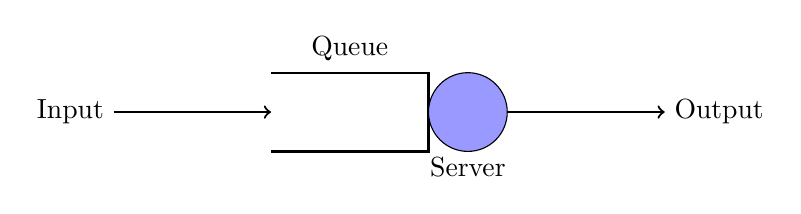
\begin{tikzpicture}
    % Draw the queue block (left-open rectangle)
    \draw[thick] (0, 0.5) -- (2, 0.5) -- (2, -0.5) -- (0, -0.5);
    \node at (1, 0.8) {Queue};

    % Draw the input arrow
    \draw[->, thick] (-2, 0) -- (0, 0);
    \node[left] at (-2, 0) {Input};

    % Draw the server (circle)
    \filldraw[fill=blue!40, draw=black] (2.5, 0) circle (0.5);
    \node at (2.5, -0.7) {Server};

    % Draw the output arrow
    \draw[->, thick] (3, 0) -- (5, 0);
    \node[right] at (5, 0) {Output};
\end{tikzpicture}
        \label{fig:simpleQblk}
        \caption{Block diagram of a simple, 1-D queue with one server and infinite capacity.}
    \end{figure}

\subsection{Terminology}
The above block diagram has a few terms used in it. A queue is formed by entities. What these entities are depends on the context provided by the application of the theory. For example, it could be jobs waiting to be executed at a server in a data center, or it could be humans waiting at a bank, or it could even be calls lined up at a call center. To address the requirements of the entity, the requirements again depend on the 

Whenever a new entity is added to the queue, we call it as an arrival event.

\subsection{Kendall Notation}
A queue is characterized by how entities arrive to it, how they depart from it, how many servers are present, and if existant, what is the maximum length of the queue limited to.

\emph{Kendall's Notation} provides a condensed way to denote a queue. The general form is given by 
\begin{subequations}
    \begin{align}
        \mX / \mY / x / y 
    \end{align}
    where, 
    \begin{align*}
        \mX &= \text{Describes arrival statistics.}\\
        \mY &= \text{Describes the departure statistics.} \\
        x &= \text{Number of Servers.}\\
        y &= \text{Maximum length of the queue.} 
    \end{align*}
\end{subequations}
A frequently used statistics is \emph{Markovian}, where the process(es) of arrival and/or departure are Markov. `M' is used to abbreviate a Markovian statistics, `D' to denote Deterministic Timing, `G' for general statistics and `Geom' for Geometric. 

\subsection{Assumptions}

\begin{enumerate}
    \item 
\end{enumerate}

\chapter{M/M/1 Queue}
In this chapter, we will study the simplest kind of queue, the $M/M/1$ or also known as \emph{Markovian} queue. While the queue, once we get to its details may not seem realistics, it does provide valuable insights due to its mathematical tractability.

\dfn{M/M/1 (or Markovian) Queue}{
    A $M/M/1$ queue, also known as \emph{Markovian} queue is characterized as follows:
    \begin{enumerate}
        \item The arrival process is a Poisson Random process.
        \item There is a single server with the serving times being exponentially distributed. 
        \item There is no limit on the size of the queue. Also, the state of the queue is given by the number of arrivals/ customers in the queue at a given moment.
    \end{enumerate}  
}

% \dfn{Limit of Sequence in }{Let be a sequence in}

% \qs{}{Is the set a closed set}
% \sol We have to take its complement and check whether that set is a open set i.e. if it is a union of open balls
% \nt{We will do topology in Normed Linear Space  (Mainly  and occasionally)using the language of Metric Space}
% \clm{Topology}{}{Topology is cool}
% \ex{Open Set and Close Set}{}

\chapter{Appendix}
Only the bare minimum concepts have been covered here. I strongly advise that you go through the relevant material in \cite{pishro2014introduction}
\section{Random Processes}
\dfn{Random Process}{A random process is a collection (or a sequence) of variables usually indexed by time.
}
If the indexing variable is continuous, we refer to the process as a continuous-time random process and if the indexing variable is discrete, we call the process a discrete-time process. Thus, sampling a random process at a time instant gives a random variable. If this random variable is discrete, we call the process a discrete-valued process. Similarly, we define continuous-valued process. 

% References :
\bibliography{references}
\bibliographystyle{plain}

\end{document}
